\begin{frame}[t,fragile]{擬似乱数発生器}
  \begin{itemize}
    %\setlength{\itemsep}{1em}
  \item 最も簡単な乱数発生器:線形合同法 (linear congruential method)
    \[
    x_{n+1} = (ax_n+c) \ \mbox{mod} \ m
    \]
  \item 例) $a = 65539$, $c = 0$, $m = 2147483648$ (周期 $m-1$)
  \item 少しだけ異なる初期値 $(x0 = 1, 2, 3)$ から始めた場合
  \resizebox{!}{.35\textheight}{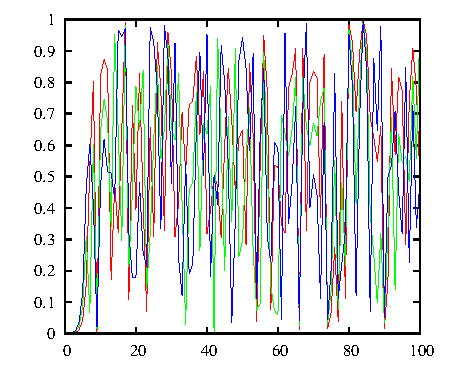
\includegraphics{image/lcg-1.pdf}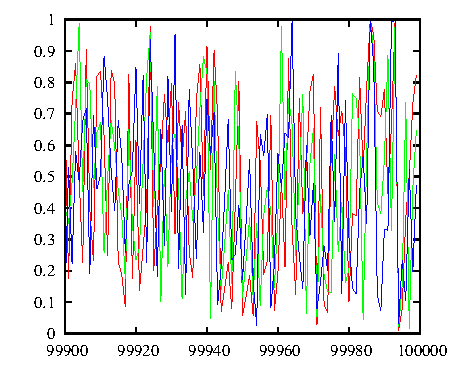
\includegraphics{image/lcg-2.pdf}}
  \item 数十ステップ進むとバラバラな振舞い ⇒ カオス的
  \end{itemize}
\end{frame}
